\PassOptionsToPackage{unicode=true}{hyperref} % options for packages loaded elsewhere
\PassOptionsToPackage{hyphens}{url}
%
\documentclass[]{article}
\usepackage{lmodern}
\usepackage{amssymb,amsmath}
\usepackage{ifxetex,ifluatex}
\usepackage{fixltx2e} % provides \textsubscript
\ifnum 0\ifxetex 1\fi\ifluatex 1\fi=0 % if pdftex
  \usepackage[T1]{fontenc}
  \usepackage[utf8]{inputenc}
  \usepackage{textcomp} % provides euro and other symbols
\else % if luatex or xelatex
  \usepackage{unicode-math}
  \defaultfontfeatures{Ligatures=TeX,Scale=MatchLowercase}
\fi
% use upquote if available, for straight quotes in verbatim environments
\IfFileExists{upquote.sty}{\usepackage{upquote}}{}
% use microtype if available
\IfFileExists{microtype.sty}{%
\usepackage[]{microtype}
\UseMicrotypeSet[protrusion]{basicmath} % disable protrusion for tt fonts
}{}
\usepackage{hyperref}
\hypersetup{
            pdftitle={An Assessment of FGCU's Learning Assistant Program},
            pdfauthor={Blake Gilliland, Advised by Dr.~Galen Papkov},
            pdfborder={0 0 0},
            breaklinks=true}
\urlstyle{same}  % don't use monospace font for urls
\usepackage[margin=1in]{geometry}
\usepackage{graphicx,grffile}
\makeatletter
\def\maxwidth{\ifdim\Gin@nat@width>\linewidth\linewidth\else\Gin@nat@width\fi}
\def\maxheight{\ifdim\Gin@nat@height>\textheight\textheight\else\Gin@nat@height\fi}
\makeatother
% Scale images if necessary, so that they will not overflow the page
% margins by default, and it is still possible to overwrite the defaults
% using explicit options in \includegraphics[width, height, ...]{}
\setkeys{Gin}{width=\maxwidth,height=\maxheight,keepaspectratio}
\setlength{\emergencystretch}{3em}  % prevent overfull lines
\providecommand{\tightlist}{%
  \setlength{\itemsep}{0pt}\setlength{\parskip}{0pt}}
\setcounter{secnumdepth}{0}
% Redefines (sub)paragraphs to behave more like sections
\ifx\paragraph\undefined\else
\let\oldparagraph\paragraph
\renewcommand{\paragraph}[1]{\oldparagraph{#1}\mbox{}}
\fi
\ifx\subparagraph\undefined\else
\let\oldsubparagraph\subparagraph
\renewcommand{\subparagraph}[1]{\oldsubparagraph{#1}\mbox{}}
\fi

% set default figure placement to htbp
\makeatletter
\def\fps@figure{htbp}
\makeatother

\usepackage{amssymb}
\usepackage{indentfirst}
\usepackage{setspace}\doublespacing
\usepackage{graphicx}
\usepackage{array}
\usepackage{booktabs}
\usepackage{multirow}
\usepackage{pdflscape}
\usepackage{float}
\usepackage{tabu}
\usepackage{threeparttable}
\newcommand*\conj[1]{\bar{#1}}
\newcommand*\mean[1]{\bar{#1}}

\title{An Assessment of FGCU's Learning Assistant Program}
\author{Blake Gilliland, Advised by Dr.~Galen Papkov}
\date{}

\begin{document}
\maketitle

\hypertarget{abstract}{%
\subsection{Abstract}\label{abstract}}

FGCU's Learning Assistant program began in 2016 and spanned a wide range
of STEM disciplines. In the last year, it has expanded to non-STEM
classes as well. We are interested in measuring the effectiveness of the
program and determining methods of improvement for the future based on
DFW rates.

\hypertarget{background}{%
\subsection{Background}\label{background}}

The Learning Assistant (LA) model is a relatively new concept. It began
at the University of Colorado at Boulder in 2003 and has spread to over
200 universities around the United States due to the success they had.
The most familiar role that one may compare an LA to is a Teacher's
Assistant (TA) or an Instructional Assistant (IA). LA's are talented
undergraduates who have recently taken a course and remember what it is
like to learn the material. However, there are significant differences
between them and TA's or IA's that allows them to be in a category of
their own. They help transform undergraduate courses to include small
groups of students articulating, defending, and modifying their ideas
about relevant problems or phenomena. Their main role is to support
student learning in interactive classroom environments, working with
small groups of students as they solve challenging conceptual or
mathematical problems. They are required to take a pedagogy course
during their first semester as an LA so they can develop their skills
and theoretical understanding of effective teaching techniques.
\cite{UC_LA} \cite{cochran}

\begin{figure}
\centering
\includegraphics{./tex2pdf.-c1091a137b26069e/3974a14292c1b9c2f61eea74b2ad90e9a9acc7e7.png}
\caption{The LA model varies significantly from a traditional
classroom.}
\end{figure}

There has been research conducted on what the impact of LA's are in the
classroom. Using Learning Assistant Supported Student Outcomes (LASSO),
a web-based learning gains assessment application that provides
validated instruments accross a range of disciplines, researchers have
been able to conduct statistical analysis on specific ways that having
an LA model can affect student performance accross various courses.

One paper entitled ``The Impact of Learning Assistants on Inequities in
Physics Student Outcomes'' gave noteworthy results. These researchers
investigated how LA's can help underrepresented minorities to succeed in
physics classes and how it stacks up to majority students. They used
pre-/post- test score on a number of exams on commmon topics accross
many different universities to determine an effect size, known in
statistics as Cohen's d. Cohen's d is a measurement of the difference
between the means of two groups, often but not always used with
before/after situations, and is used when the groups have similar
standard deviations. They implemented other types of analyses including
predictive models for outcomes and other student performance metrics.
Many of the results were statistically significant indicating that LA's
seriously help underrepresented minorities to be more successful in
physics courses. \cite{VanDusen1}

Another paper entitled ``LASSO Study Initial Findings'' is a report on
some research done accross disciplines and universities comparing
student outcomes in courses with LA's to those without them. They did
pre-/post-tests using surveys with topics from concept inventories
including chemistry, physics, biology, and genetics. The questions they
wanted to answer are as follows:

\begin{enumerate}
\def\labelenumi{\arabic{enumi}.}
\tightlist
\item
  How do teachers' uses of LA's predict student performance in LA
  supported courses, if at all?
\item
  How do course attributes predict student performance in LA supported
  courses, if at all?
\item
  How do students' attributes predict student performance in LA
  supported courses, if at all?
\item
  How do students' interactions with LA's predict student performance in
  LA supported courses, if at all?
\end{enumerate}

They had a number of statistically significant results which included
females having a statistically significantly lower effect size than
males (Cohen's d), and that the average effect sizes for white students
were statistically significantly different from Asian, black, and
``other'' students. Also, ``students average effect size increases with
the amount of time they spend with LAs. The trend peaks at 16-30
minutes/week, which is also the only category to be statistically
significant from the 0 minutes/week category.'' There were other
significant outcomes, as well. \cite{VanDusen2}

Florida Gulf Coast University (FGCU) has been running their LA program
since 2016 with the help of
\href{mailto:Noyce@FGCU}{\nolinkurl{Noyce@FGCU}}, a grant awarded in
2015 to the university to help encourage STEM majors to pursue teaching
careers. The intent of \href{mailto:Noyce@FGCU}{\nolinkurl{Noyce@FGCU}}
was to build a lasting pipeline of talented STEM students from
underrepresented groups to meet the growing needs of diverse Southwest
Florida school districts. The program's mission was, and still is, to
recruit undergraduate STEM majors in Biology, Chemistry, Mathematics,
and Engineering, and to prepare them to become grades 6-12 Science or
Math teachers. The Noyce Scholars undertake an Education Minor and
become certified teachers at high needs public schools. They wanted to
increase the number of STEM classroom teachers for grades 6--12 by
producing qualified STEM teachers for filling critical shortages of math
and science teachers in Southwest Florida. \cite{johnson}

Similarly, they were interested in increasing the success of
\href{mailto:Noyce@FGCU}{\nolinkurl{Noyce@FGCU}} classroom teachers
through preservice enrichment, first-year mentoring by an in-school
teacher, and having a first-year in service coach. They support teacher
certification of \href{mailto:Noyce@FGCU}{\nolinkurl{Noyce@FGCU}}
scholars so that they complete certification testing before graduation,
including support through cooperation with the school districts for a
successful completion of the first-year of professional teaching.

Beginning in the fall of 2019, the Office of Undergraduate Scholarship
began funding the program. Appropriately, they wanted to carefully
examine the LA program and make sure that it was reaching its goals of
improving student performance. There are some outstanding questions that
there are not answers to yet locally. From the aforementioned previous
research, it is clear that the LA model has serious upside and our
program would like to see similar results. While we do not currently
have nearly the resources and data that these other research projects
have used, we do have basic indicators as a starting point. In the
future, we wish to be able to answer more sophisitcated and intricate
questions regarding the health and effectiveness of the program,
particularly when it comes to its effect on minorities and differences
between females and males. The questions we wish to consider in this
paper are as follows:

\begin{enumerate}
\def\labelenumi{\arabic{enumi}.}
\tightlist
\item
  Do D/F/Withdrawl (DFW) rates among all subject areas improve when an
  LA is present compared to when they are not?
\item
  Do DFW rates among classes with the same instructor improve when an LA
  is present compared to when they are not?
\end{enumerate}

\hypertarget{methodology-analysis}{%
\subsection{Methodology \& Analysis}\label{methodology-analysis}}

Our goal is to see how DFW are affected by instituting the LA model. We
collected data describing these rates accross a total of 18 courses that
had sections with and without an LA using Tableau.

\begingroup\fontsize{7}{9}\selectfont

\begin{longtable}{llrr}
\toprule
LA & Course & DFW Count & DFW Rate\\
\midrule
\endfirsthead
\multicolumn{4}{@{}l}{\textit{(continued)}}\\
\toprule
LA & Course & DFW Count & DFW Rate\\
\midrule
\endhead
\
\endfoot
\bottomrule
\endlastfoot
\rowcolor{gray!6}  No & Calculus I & 124 & 0.33\\
Yes & Calculus I & 39 & 0.28\\
\rowcolor{gray!6}  No & Calculus II & 26 & 0.20\\
Yes & Calculus II & 12 & 0.34\\
\rowcolor{gray!6}  No & College Algebra & 784 & 0.28\\
\addlinespace
Yes & College Algebra & 88 & 0.31\\
\rowcolor{gray!6}  No & College Physics w/Lab II & 5 & 0.16\\
Yes & College Physics w/Lab II & 5 & 0.16\\
\rowcolor{gray!6}  No & Elementary Calculus & 76 & 0.35\\
Yes & Elementary Calculus & 50 & 0.47\\
\addlinespace
\rowcolor{gray!6}  No & Engineering Mechanics & 14 & 0.27\\
Yes & Engineering Mechanics & 6 & 0.16\\
\rowcolor{gray!6}  No & Finite Mathematics & 23 & 0.11\\
Yes & Finite Mathematics & 18 & 0.17\\
\rowcolor{gray!6}  No & Gen'l Biology w/Lab I & 477 & 0.34\\
\addlinespace
Yes & Gen'l Biology w/Lab I & 40 & 0.35\\
\rowcolor{gray!6}  No & General Chemistry I & 682 & 0.37\\
Yes & General Chemistry I & 178 & 0.39\\
\rowcolor{gray!6}  No & General Chemistry II & 138 & 0.33\\
Yes & General Chemistry II & 152 & 0.41\\
\addlinespace
\rowcolor{gray!6}  No & Intermediate Algebra & 464 & 0.22\\
Yes & Intermediate Algebra & 62 & 0.29\\
\rowcolor{gray!6}  No & Intro Earth Science & 47 & 0.15\\
Yes & Intro Earth Science & 22 & 0.16\\
\rowcolor{gray!6}  No & Intro to Computer Science & 36 & 0.22\\
\addlinespace
Yes & Intro to Computer Science & 31 & 0.17\\
\rowcolor{gray!6}  No & Intro. Environmental Science & 13 & 0.09\\
Yes & Intro. Environmental Science & 3 & 0.08\\
\rowcolor{gray!6}  No & Introduction to Programming & 6 & 0.12\\
Yes & Introduction to Programming & 21 & 0.13\\
\addlinespace
\rowcolor{gray!6}  No & Precalculus & 211 & 0.25\\
Yes & Precalculus & 53 & 0.22\\
\rowcolor{gray!6}  No & Social Science Statistics & 12 & 0.18\\
Yes & Social Science Statistics & 5 & 0.16\\
\rowcolor{gray!6}  No & Statistical Methods & 674 & 0.25\\
\addlinespace
Yes & Statistical Methods & 23 & 0.21\\*
\end{longtable}
\endgroup{}

As mentioned, we wish to be able to answer the question of whether DFW
rates improve (decrease) when an LA is present compared to when they are
not. Due to limitations with the data, i.e.~not having as much of it as
we would have liked (n \(\approx\) 30), we need to perform a
Shapiro-Wilk Normality test. This test will take in the data, examine
its shape relative to the number of data points, and determine if it is
normal \emph{enough} to use parametric tests. The Shapiro-Wilk Normality
test would not be appropriate to use when having larger data sets. We
will perform the test on the difference between the LA DFW rates and the
Non-LA DFW rates since what we are interested in is whether DFW rates in
LA courses are lesser than the alternative.

Our hypothesis is that the data is normal and thus a significant p-value
would indicate non-normal data. Shapiro-Wilk Normality test for DFW
Rates accross sections (with and without LA's) (\(\alpha = .05\)), along
with a histogram of the data being tested:

\begin{verbatim}
## 
##  Shapiro-Wilk normality test
## 
## data:  tab3$`DFW Rate`[tab3$LA == "Yes"] - tab3$`DFW Rate`[tab3$LA ==     "No"]
## W = 0.97381, p-value = 0.8655
\end{verbatim}

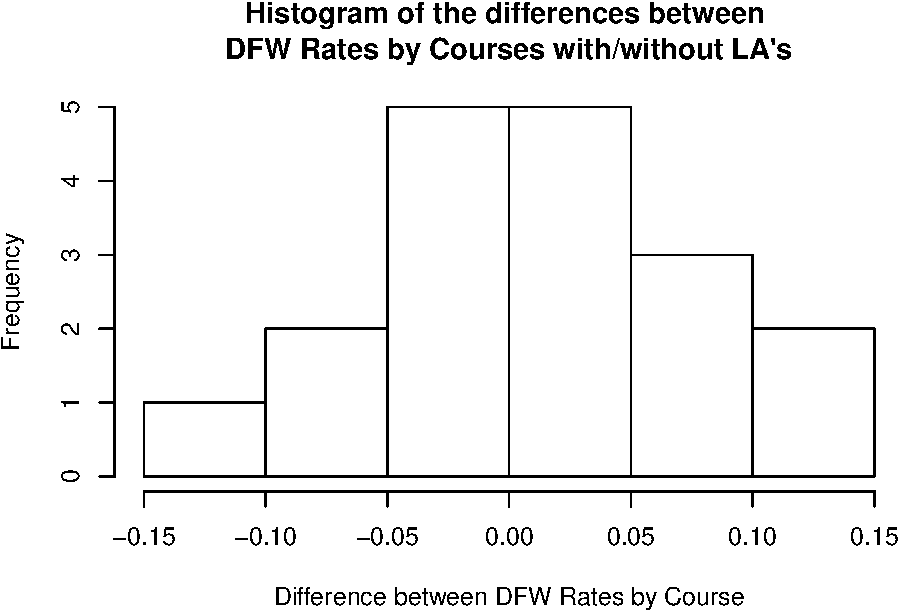
\includegraphics{./tex2pdf.-c1091a137b26069e/b93c8366305c29630c969a7163cce6008d4d0cd9.pdf}

Since we have a p-value of p = .8655, we fail to reject our hypothesis
and thus we have evidence to conclude the difference between DFW rates
for courses with and without LA's does follow an approximately normal
distribution.

We may now proceed with our testing. We choose to employ a left tailed,
two-sample, paired, t-test for differences in DFW rates accross sections
based on presence of LA's (\(\alpha = .05\)). We test against the
hypothesis that DFW rates in courses with LA's are equivalent to that of
non-LA courses.

\begin{verbatim}
## 
##  Paired t-test
## 
## data:  LA_DFW and NonLA_DFW
## t = 0.8984, df = 17, p-value = 0.8092
## alternative hypothesis: true difference in means is less than 0
## 95 percent confidence interval:
##       -Inf 0.0391512
## sample estimates:
## mean of the differences 
##              0.01333333
\end{verbatim}

We observe a test statistic of t = .8984 and an associated p-value of p
= .8092. Thus we fail to reject the hypothesis that there are no
differences in DFW rates among courses with LA's compared to those
without them. This definitely is not the desired result from the LA
Program's point of view. Even though the p-value is not significant in
either direction, it is noteworthy that we do not even observe a
decrease in the mean difference between rates of LA and non-LA courses.
In other words, the mean DFW rate in non-LA courses
(\(\bar{x_{non}} = .23\)) is lower than that of LA courses
(\(\bar{x_{LA}} = .25\)).

For LA courses to have significantly lower DFW rates, the density would
need to be shifted considerably leftward. As is, our distributions are
remarkably similar in shape and location.\(\\\)

{}

As can be seen in the density plot above, the distribution of DFW rates
for both groups are very similar. For LA's to be seen as more effective,
the respective density would need a significant leftward shift.

We would also like to examine the DFW rates in a different context.
Accross courses, as we have just discussed, was the most obvious and
broad way to compare LA courses to Non-LA courses. However, there are
issues with it such as not being able to account for different teaching
styles and abilities of instructors in those courses among other things.

We will filter our courses by instructor and pair on LA and Non-LA
courses. The courses will still be separated, however. In other words,
we will compare LA and Non-LA DFW rates by pairing instructors who have
taught the same course with and without LA's. This way we can account
for teaching style and mitigate that variance. We will assign
instructors a number for anonymity.

\begingroup\fontsize{7}{9}\selectfont

\begin{longtable}{lrrr}
\toprule
LA & Instructors & DFW Count & DFW Rate\\
\midrule
\endfirsthead
\multicolumn{4}{@{}l}{\textit{(continued)}}\\
\toprule
LA & Instructors & DFW Count & DFW Rate\\
\midrule
\endhead
\
\endfoot
\bottomrule
\endlastfoot
\rowcolor{gray!6}  No & 1 & 25 & 0.32\\
Yes & 1 & 27 & 0.36\\
\rowcolor{gray!6}  No & 2 & 19 & 0.26\\
Yes & 2 & 21 & 0.30\\
\rowcolor{gray!6}  No & 3 & 25 & 0.17\\
\addlinespace
Yes & 3 & 42 & 0.29\\
\rowcolor{gray!6}  No & 4 & 2 & 0.06\\
Yes & 4 & 3 & 0.09\\
\rowcolor{gray!6}  No & 5 & 13 & 0.23\\
Yes & 5 & 13 & 0.23\\
\addlinespace
\rowcolor{gray!6}  No & 6 & 29 & 0.33\\
Yes & 6 & 25 & 0.28\\
\rowcolor{gray!6}  No & 7 & 20 & 0.56\\
Yes & 7 & 11 & 0.16\\
\rowcolor{gray!6}  No & 8 & 42 & 0.49\\
\addlinespace
Yes & 8 & 45 & 0.48\\
\rowcolor{gray!6}  No & 9 & 6 & 0.08\\
Yes & 9 & 3 & 0.08\\
\rowcolor{gray!6}  No & 10 & 5 & 0.16\\
Yes & 10 & 5 & 0.16\\
\addlinespace
\rowcolor{gray!6}  No & 11 & 29 & 0.54\\
Yes & 11 & 50 & 0.47\\
\rowcolor{gray!6}  No & 12 & 5 & 0.16\\
Yes & 12 & 5 & 0.16\\
\rowcolor{gray!6}  No & 13 & 45 & 0.48\\
\addlinespace
Yes & 13 & 45 & 0.49\\
\rowcolor{gray!6}  No & 14 & 6 & 0.19\\
Yes & 14 & 14 & 0.20\\
\rowcolor{gray!6}  No & 15 & 14 & 0.16\\
Yes & 15 & 10 & 0.19\\*
\end{longtable}
\endgroup{}

Again, we do not have enough data to assume using parametric tests would
be appropriate so a Shapiro-Wilk test is used to determine if a
nonparametric approach would be the appropriate route to take. As before
with the by-course data, we will perform the test on the differences
between the by-instructor DFW rates (\(\alpha = .05)\):

\begin{verbatim}
## 
##  Shapiro-Wilk normality test
## 
## data:  tab3$`DFW Rate`[tab3 == "Yes"] - tab3$`DFW Rate`[tab3$LA == "No"]
## W = 0.63002, p-value = 4.869e-05
\end{verbatim}

{}

Our p-value, which is nearly 0, is less than \(\alpha = .05\) thus we
may conclude that the differences between DFW rates controlled by
instructor is not approximately normally distributed. As a result, we
will use a nonparametric test to test for differences.

A left-tailed, two-sample, and paired Wilcoxon Signed-Rank test will be
used to test against the hypothesis that the average DFW rate in LA
courses is equivalent to that of Non-LA courses (\(\alpha = .05\)).

\begin{verbatim}
## 
##  Wilcoxon signed rank test with continuity correction
## 
## data:  LA_DFW and NonLA_DFW
## V = 36, p-value = 0.6225
## alternative hypothesis: true location shift is less than 0
\end{verbatim}

With a p-value of p=.6225, we fail to reject our hypothesis that the
differences between DFW rates between courses controlled by instructor
with/without LA's is in the favor of LA courses. \(\\\)

{}

\hypertarget{conclusions-interpretations-considerations}{%
\subsection{Conclusions, Interpretations, \&
Considerations}\label{conclusions-interpretations-considerations}}

We have seen from our analysis, be it limited due to limitations on data
availability and integrity, that there is not evidence to conclude that
having a Learning Assistant in the class room is having a positive
effect on students' ability to pass courses. However, it is our
conjecture that there is reason to believe that there are underlying
truths in the data that were not represented in the data due to lack of
foresight when recording the data. For example, courses with a Learning
Assistant had only one and no Instructional Assistants. However, courses
with no Learning Assistants may have had an Instructional Assistant. So,
in our Non-LA data we may have had courses who had an assistant in the
classroom who, though not having the role of a Learning Assistant, could
be trained as one and is utilizing the techniques they have learned in
the pedagogy course. This would cause a leftward shift in the DFW rates.
Going forward, when recording data we will account for all types of
assistants participating in the course.

Another consideration for why we do not see significant differences is
lack of training. Instructors may participate and self-select Learning
Assistants without ever going through rigorous training on how Learning
Assistants are to be utilized in the classroom. Most do not restructure
the classroom by forming the small groups and raising classtime
interaction. Simply, Learning Assistants are being used as Instructional
Assistants. This defeats the point of the Learning Assistant program.

Can we do better with our data? Are DFW rates the best indicator for
Learning Assistant impact on student performance? Perhaps not. This too
could account for lack of differences.

Too, an issue that cannot be ignored: lack of funding and support from
the university, many participating faculty in the program have
expressed, limits the program's ability to train participating members
and implement the structure and policies that universities with growing
programs have. There is a desperate need to thoroughly train instructors
on how to commit and transition to a new classroom structure. Learning
Assistants need to have a similar program in addition to the pedagogy
course. Funding for trips to the Learning Assistant program conferences
around the country need to be available so that the spread of ideas is
reaching FGCU.

\hypertarget{future-research}{%
\subsection{Future Research}\label{future-research}}

As mentioned, the data needs to be better. Collection and recording
techniques must improve to have data with higher integrity, as well as
more kinds of data to do a wider and more thorough analysis on. There
are many analyses and data collection approaches from the literature
available that is worth looking into for future prospects. Making use of
LASSO would have a clear positive effect on improving the quality of
data. Implementing pre-/post- exams for all LA based courses that come
from a concept inventory would be an effective constant to limit
variability in results. \cite{VanDusen1}

As far as analysis goes, once that data is obtained, we would like to do
more predictive modeling than inferential statistics. Currently, we are
implementing a multiple multivariate linear regression model to predict
student grades regressed on instructor, presence of an LA, the term the
course is in, and what the course is. So, this goes further than simple
DFW rates. It will get at exact grades to see if passing students
potentially pass at a higher level with an LA than those who do not have
one. But after this we would like to do more with comparing differences
between LA effects on sexes (male/female), ethnicity, college
generation, as well. \cite{VanDusen2}

Though overall the analysis we have conducted did not give results in
favor of the LA program, there is consolation by a few of the courses
such as Introduction to Computer Science (COP 1500) and Introduction to
Programming (COP 2006). For years these classes have been on the cutting
edge of involving Learning Assistants and have seen great results in the
form of extremely low DFW rates. We plan to examine these courses more
thoroughly for differences between and their Non-LA counterparts in
hopes of implementing some of the techniques used in those classrooms.

\hypertarget{acknowledgements}{%
\subsection{Acknowledgements}\label{acknowledgements}}

Thank you to Dr.~Galen Papkov for mentoring me through the research
process and giving me guidance on using R to perform the analysis and R
Markdown to create the report.

I also would like to thank the Office of Undergraduate Scholarship as
well as Dr.~Katie Johnson for giving me the opportunity to take the
reigns on this research, giving me a perfect balance of guidance and
autonomy for the direction we wanted to take the analysis in.
Dr.~Charles Gunnels, the head of the office, was instrumental in
obtaining the data and providing a vision that will be used on into the
future for the goal of strengthening the Learning Assistant program.

\bibliographystyle{plain}
\bibliography{ref}

\end{document}
